% !TEX root = ../../../main.tex

\chapter{Piano di indirizzamento IP}

\section{VLAN}
I dispositivi scelti hanno dei preset per la creazione di VLAN. Nello specifico, per le tre reti
richieste, si utilizzerà un preset di tipo ``Corporate'', il quale consente la comunicazione tra
reti virtuali differenti. Si potrà successivamente creare una rete di tipo ``Guest'' isolata da queste.

La console consente la gestione di queste reti virtuali mediante un'interfaccia grafica in cui si
possono configurare gli switch presenti, porta per porta. Inoltre, nonostante venga teoricamente effettuato in maniera
automatica, è possibile assegnare un range di indirizzi IP per ogni VLAN, divisi per router.

Per la rete ``Guest'' si porrà un numero di indirizzi fissi assegnabili alle prese del tavolo
della sala riunioni, ma non sapendo il numero di utenti connessi alla futura rete WLAN, si consiglia di
impostare gli access point con degli indirizzi pubblici, ma effettuanti NAT per tutti i dispositivi a loro connessi.

Se si desidera visualizzare una simulazione della schermata di configurazione di un sistema simile,
visitare il sito \url{demo.ui.com}. La creazione di nuove reti virtuali è disponibile nella parte di
impostazioni accessibili dall'icona in basso a sinistra, nella sezione ``Networks''.

\begin{table}[ht]
  \begin{adjustbox}{center}
    \begin{tabular}{@{}lll@{}}
      \toprule
      Subnet             & Range                     & Utilizzo                  \\ \midrule
      196.111.250.0/26   & \begin{tabular}[c]{@{}l@{}}196.111.250.1 - 196.111.250.62\\ 196.111.250.63 Broadcast\end{tabular} & \begin{tabular}[c]{@{}l@{}}Riservata per la gestione della rete.\\Una parte di questa subnet\\(isolata con mod. Guest)\\sarà dedicata collegamento ospiti.\end{tabular} \\
      196.111.250.64/26  & \begin{tabular}[c]{@{}l@{}}196.111.250.65 - 196.111.250.126\\ 196.111.250.127 Broadcast\end{tabular} & LAN amministrazione       \\
      196.111.250.128/26 & \begin{tabular}[c]{@{}l@{}}196.111.250.129 - 196.111.250.190\\ 196.111.250.191 Broadcast\end{tabular} & LAN produzione            \\
      196.111.250.192/26 & \begin{tabular}[c]{@{}l@{}}196.111.250.193 - 196.111.250.254\\ 196.111.250.255 Broadcast\end{tabular} & LAN sperimentale          \\ \bottomrule
    \end{tabular}
  \end{adjustbox}
  \caption{Il piano di indirizzamento generale.}\label{tab:piano-ind-generale}
\end{table}

\newpage
\subsection{Subnetting}
Dato che è stato specificato un numero massimo di 62 indirizzi pubblici per subnet, si sceglie di
utilizzare una netmask da 26 bit. In questo modo, 2 bit identificheranno il numero di rete ed altri
6 saranno disponibili per 64 indirizzi IP.

Nello specifico, fare riferimento al seguente schema:

\begin{figure}[ht]
  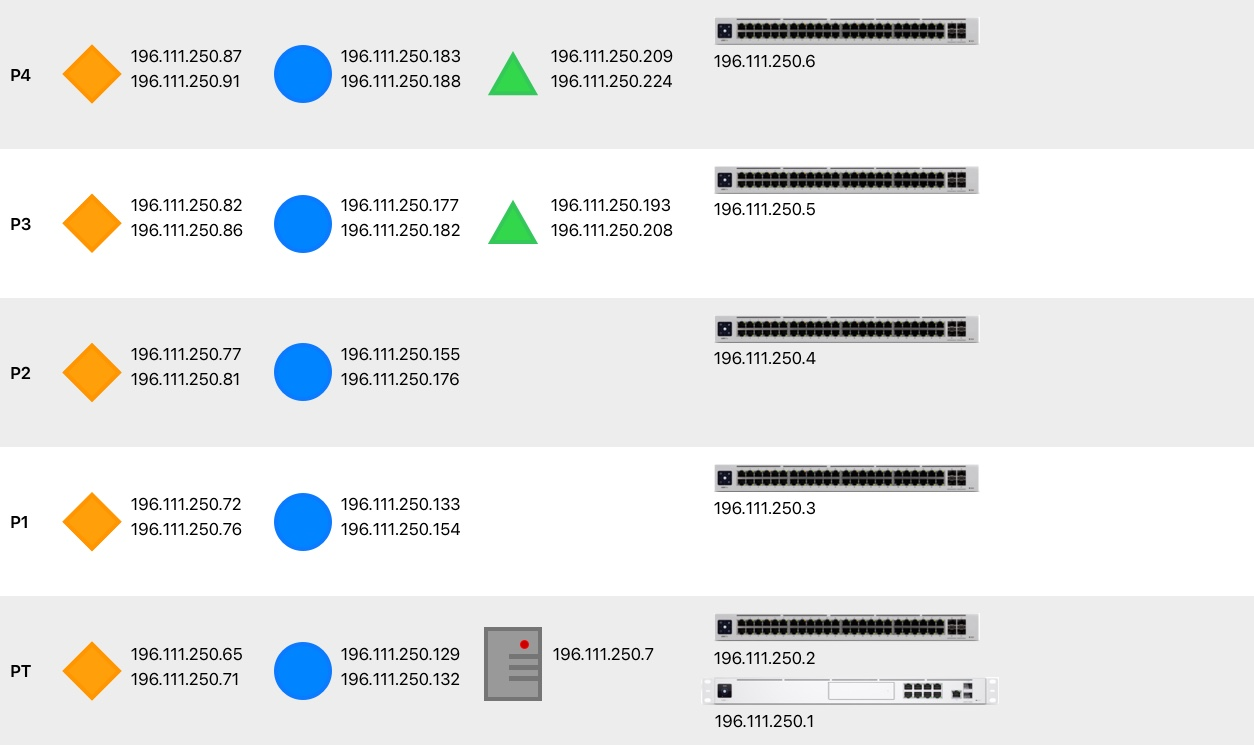
\includegraphics[width=\textwidth]{indirizzamento.jpg}
  \caption{Il piano di indirizzamento complessivo. Rombo: LAN amministrazione, cerchio: LAN produzione, triangolo: LAN sperimentale.}\label{fig:indirizzamento}
\end{figure}

Per eventuali server futuri aggiuntivi, si suppone che assumano degli indirizzi IP sequenziali rispetto al primo.

La soluzione presentata, in cui ogni postazione assume un indirizzo IP pubblico, richiede una particolare attenzione
dal punto di vista della sicurezza. Occorrerà impostare il gateway (il quale implementa funzionalità di sicurezza) in modo
da filtrare eventuali connessioni rischiose dall'esterno, come potenziali attacchi. Potrebbero essere necessari dei dispositivi
aggiuntivi, ma questo è al di fuori dello scopo di questa relazione.

La soluzione si presenta molto comoda nel caso in cui sia necessario avere accesso da remoto a tutte le macchine, si pensi ad esempio
alla semplicità con cui si può ricevere assistenza oppure accedere a computer ed altre strumentazioni anche lavorando da casa o fuori sede.